\documentclass[12pt,a4paper]{article}
\usepackage{graphicx}
\usepackage{biblatex}
\usepackage{parskip}
\usepackage{listings}
\usepackage{pdfpages}
\usepackage{rotating}
\usepackage{pdflscape}
\usepackage{amsmath}
\usepackage{subcaption} 
\usepackage{setspace}

\lstset{%
basicstyle=\ttfamily,
breaklines = true,
tabsize=2
}
\graphicspath{ {./Images/} }
\addbibresource{biblography.bib}

\setlength{\parskip}{1em}
\begin{document}

\begin{titlepage}
	\newcommand{\HRule}{\rule{\linewidth}{0.5mm}}
    
\includegraphics[width = 4cm]{./Images/Logo.jpg}\\[0.5cm] 
    
    \center 
	\textsc{\large Information Processing }\\[0.3cm] 
    
	\HRule \\[0.3cm]
	Coursework Report
    \HRule \\[0.7cm]
     
    \begin{center}
		\underline{Authors}\\[0.1cm] Brandon Cann\\[0.1cm]
        Vajiravidh Pongpaew\\[0.1cm]
        David Maël\\[0.1cm]
        Petra Ratkai\\[0.1cm]
		Razvan Rusu\\[0.1cm]
		Thomas van Issum\\[0.7cm]
	\end{center} \large

    \tableofcontents

    \vfill % Fill the rest of the page with whitespace
\end{titlepage}

\section{\normalsize System Purpose}

{\scriptsize The IoT system we have designed is a points-based racing game. 
It currently supports 6 players; however, this could readily be 
scaled up to facilitate more players. The FPGA is primarily used 
as a steering wheel for the game, however the score of each player 
is also displayed on the FPGA’s 7-segment display. The game itself 
is hosted on an HTTP server that each player can connect to using a 
web browser. Each player controls their vehicle by moving their FPGA 
and at the same time they can see their vehicle’s movements once 
connected to the server. Players can see a map of the course with 
various terrain, as well as their relative position compared to 
other vehicles and scores. Each player has a finite number of “lives” 
after which they will no longer be able to gain any points and their 
vehicle will disappear. The course itself consists of several different 
terrain types, represented by different coloured tiles. The FPGA 
receives the type of terrain its vehicle is on and processes the 
accelerometer data, in order to represent the differing responsiveness 
of driving on different types of terrain in real life. }

\section{\normalsize System Architecture}

{\scriptsize Our system consists of four nodes. The first and most important is the 
FPGA, which serves as the primary method of user interaction with the 
game. The players can move the FPGA which uses an accelerometer to quantify 
the movement data. Subsequently, the FPGA uses an FIR filter to make this 
data usable to control the vehicles. This data is then sent to the next node, 
the host PC via a JTAG UART connection. At the same time, the FPGA receives 
data from the host PC regarding the relevant vehicle’s current score as well 
as the type of terrain the vehicle is currently driving over. The FPGA displays 
its current score on its 7-segment display and uses the terrain type to select 
what type of filtering it uses. The filtering is intended to represent the 
difficulty and lack of responsiveness of driving over certain types of terrain 
e.g., ice or mud as compared to a racetrack.
\par
The two intermediary nodes are the host PC and the TCP server. The host PC’s 
primary purpose is to transfer data to and from the FPGA as well as the TCP 
server. It receives data from the FPGA and transfers data to the FPGA using 
C code that utilises the JTAG UART connection. Similarly, the host PC transfers 
data to and from the TCP server using a python script that takes the data from 
the C code. The TCP server serves a similar role to the host PC as an intermediary, 
transferring data between the host PC and the HTTP server (which is the final node). 
Specifically, the TCP server has an array of connections that continuously listen 
to the incoming data at the port. Whenever a new client connects it is added to 
this vector and the TCP server subsequently forwards the data to the HTTP server. 
The TCP and HTTP server were both implemented using Nodejs, because its flexible, 
lightweight, and fast which are all desirable characteristics for the servers.   
\par
A HTTP server was implemented as it can easily serve a webpage to a browser, 
whilst a TCP cannot. The HTTP server hosts the game and serves a html page to 
a browser. This is subsequently decoded by the browser to visually represent 
the game. The server receives the x and y position generated by the accelerometer 
and filtering of the FPGA, which it subsequently uses to identify which tile each 
vehicle will move to in the next server tick. Simultaneously, the server identifies 
the terrain and score of each vehicle, which it transfers to the TCP server so that 
it can be transferred back to the FPGA to direct filtering selection. The HTTP 
server also keeps track of the current number of lives of each player to identify 
when they have “died” and can no longer accumulate score. Finally, the server tracks 
the all-time high score via use of an external database MongoDB. MongoDB is a NOSQL 
database that can be hosted in the cloud. It was chosen because it frees up system 
resources on AWS whilst also being fast and performant. Finally, as a NOSQL database, 
it stores entries as JSON 'documents' allowing them to be easily manipulated by the 
HTTP Server. This database can be readily expanded to store other data in future. 
\par
Finally, whilst not technically a node of the system, it is possible for anybody to 
independently connect to the HTTP server, to see the visual representation of the 
game. This can be either a player or a spectator. Beyond the map itself, people 
connected to the HTTP server can also see the player scores and the all-time high 
score as can be seen in the following image:}
\par
\begin{figure} [h!]
    \centering
    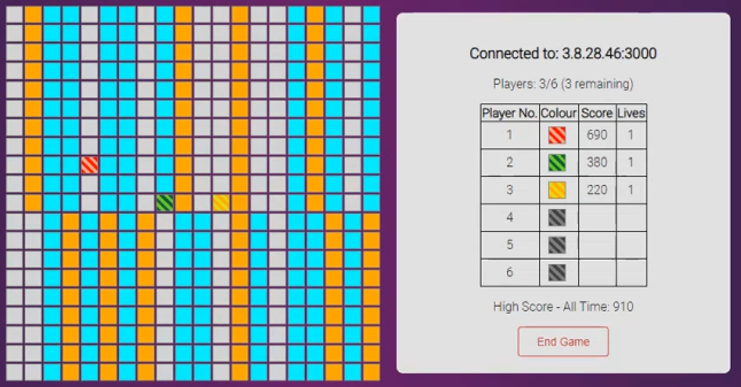
\includegraphics[scale = 0.75]{Website.png}
\end{figure}
\par
\underline{\scriptsize Diagram of Architecture}
\par
\begin{figure} [h!]
    \centering
    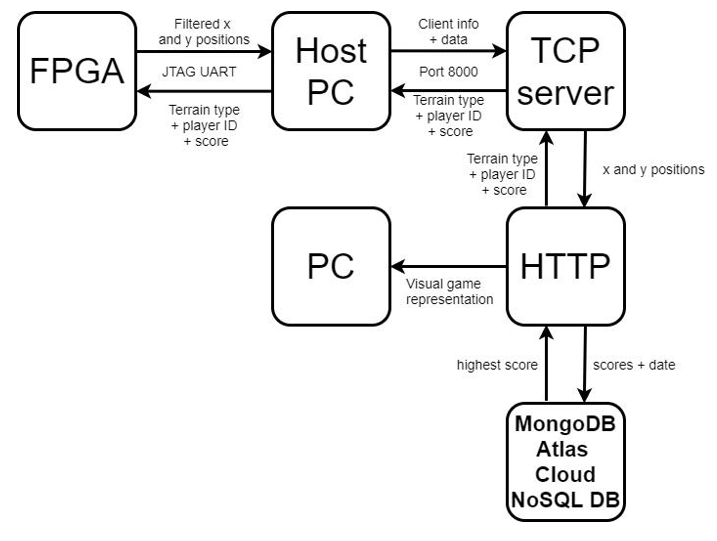
\includegraphics[scale = 0.75]{Arch.png}
\end{figure}

\section{\normalsize Performance Metrics}

{\scriptsize There are a wide variety of performance metrics that can be used given the multi-
faceted nature of the project. Several key metrics were identified: Tick rate of 
server, ping from host PC to server, connection time from host PC to FPGA, the 
processing time of the FPGA itself and finally the accuracy of the driving of 
the vehicle. These criteria are together capable of providing a comprehensive 
measurement of the system. 
\par
The processing time of the FPGA itself is evidently a critical measurement as we 
are reliant on the FPGA to fundamentally produce the data that the entire system 
is reliant on. If this were to take too long, then the system would be rendered 
pointless. There is a myriad of methods to implement the processing that all have 
a variety of trade-offs. Some methods considered were using a dedicated hardware 
FIR filter as opposed to a filter implemented in a softcore processor. Our project 
instead chose to focus on using a softcore processor filter, but within this there 
are still multiple implementations. Specifically, either using a floating-point 
implementation or a fixed-point implementation. The timing data for this can be 
seen below, ultimately the fixed-point was significantly faster. This implementation
 did have the trade-off of producing less precise data, however this was not a 
 problem as the precision of the data only required to differentiate between which 
 tile out of the 9 tiles the vehicle will move to. For this reason, it was decided 
 to use a fixed-point implementation as it had a superior processing time, and the 
 drawbacks were not significant. Finally, these FIR filters are designed using a 
 sampling frequency of 10Hz, this is acceptable as it is significantly higher than 
 the tick rate of the game server, whilst limiting the amount of processing done by 
 the FPGA.
 \par
 \begin{figure} [h!]
    \centering
    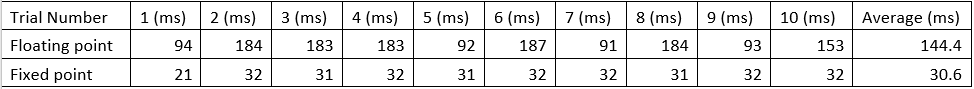
\includegraphics[scale = 0.5]{Point.png}
 \end{figure}
 \par
 Whilst the connection time from the FPGA to the host PC is potentially not as 
 critical as the processing time itself, it still can potentially serve as a 
 large delay, and thus impact the quality of the game itself. The testing data 
 for this can be seen below, but it was observed that changing the type or amount 
 of the data did not significantly impact the time taken to receive a response. 
 Therefore, the project transferred relatively more data to improve the overall 
 quality of the game without negatively impact the lag in playing the game. 
 \par
 \begin{figure} [h!]
    \centering
    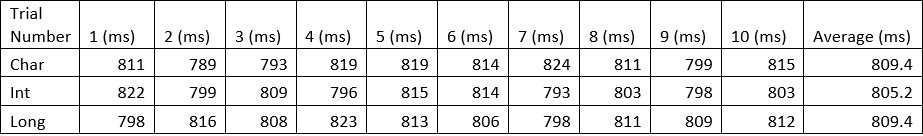
\includegraphics[scale = 0.5]{Type.png}
 \end{figure}
 \par
 The ping from the host PC to the server is relatively hard to influence directly, 
 but the quality of the transferred data itself must also be measured and maintained. 
 This metric is largely dependent on the location of the host PC’s and the server, 
 and the internet speed the host PCs are using. Therefore, the server was hosted in 
 London, a central location relative to most host PCs. This served to minimise the 
 ping from the host PC to the server, the data for which can be seen below.}
 \begin{figure} [h!]
    \centering
    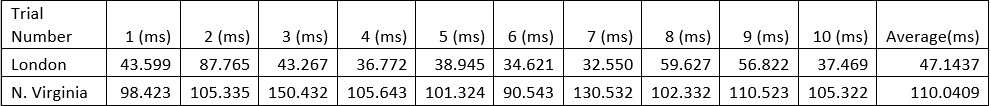
\includegraphics[scale = 0.5]{Ping.png}
 \end{figure}
 {\scriptsize The tick rate of the server is one of the most integral metrics to the game itself, 
 it dictates how accurately the game can utilise the data it receives as well as how 
 the user experiences the game. Whilst there is a theoretical maximum tick rate, the 
 data for which can be seen below, this was largely irrelevant in deciding the tick 
 rate. If the server’s tick rate was increased too much then it would be unable to 
 handle all 6 players connecting simultaneously, furthermore due to the difference 
 in the time between data from the FPGA being received and the players being able to 
 see the game on the HTTP server, if the tick rate was increased too much it could 
 become significantly harder to accurately predict the upcoming terrain and change 
 the “driving” to accommodate. Conversely if the tick rate were lower than 1Hz the 
 game would be relatively unresponsive and slow-paced drastically reducing the 
 player’s enjoyment.}
 \par
 \begin{figure} [h!]
    \centering
    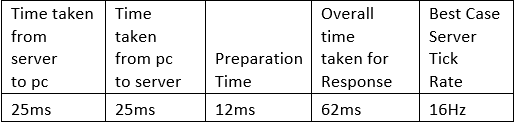
\includegraphics[scale = 0.75]{Tick.png}
 \end{figure}
 \par
 {\scriptsize Finally, the accuracy of driving the vehicle is critical to the player experience 
 of the game, despite this however there is not a quantifiable metric that can be 
 directly measured. Instead, this was tested by using a variety of different players 
 and filters to ensure that the responsiveness of the vehicle was suitable for 
 meaningfully playing the game.}

\section{\normalsize Design Decisions}

{\scriptsize There were two main design decisions in the project. The first was the visual aspect 
of the game, which was critical to the project. This must be clear and understandable 
at first glance, as well as be able to convey a lot of information such as where the 
player’s vehicle is, what the players score is, how many lives the player has, and 
the actual terrain around the player’s vehicle. Without this information a player 
would be unable to meaningfully play this game and so ensuring that it can be easily 
understood is incredibly important. Furthermore, this visual representation would 
need to be supported on a variety of monitors and web browsers. All these 
considerations had to be carefully balanced against the functional capabilities 
of the server. This led to a design that had large distinctly coloured tiles to 
represent the terrain of the course as well as clear colours to represent each 
vehicle. These colours were specifically selected to ensure red-green colour 
blindness compatibility.  Furthermore, there is a clear scoreboard to the right of 
the course that indicates each player's score as well as their remaining number of lives.
\par
The second design decision was how sensitive to make the controller and server. The 
sensitivity had to be such that tiny movements would not impact the overall movement 
of each player’s vehicle but also that players would not need to make huge movements 
to see a meaningful response. This was done in two main ways, the first is the actual 
FIR filters implemented FPGA board, whilst the data is filtered differently according 
to the terrain, each filter endeavours to minimise the impact of small movements. 
Furthermore, the server uses the direction of each movement and does not significantly 
consider the magnitude of each movement, thus ensuring that controlled movements are 
sufficient to control the vehicle. }

\section{\normalsize Testing}

{\scriptsize Initial testing was done by testing each component of the IoT system individually. 
This ensured that any errors or optimisations that could be performed on any 
individual component were all completed before it encountered any other components. 
This has the obvious benefits of being able to identify specific issues early in 
the design process and ensure that debugging them is simpler as there is no confusion 
as to which component was causing it. Similarly, it meant that each component could 
be optimised independently of other components and therefore that future trade-offs 
in terms of processing location could be tracked more easily. After this each 
connection between components was tested individually and debugged once again making 
it apparent where any errors were occurring. Finally, once the entire project was 
connected, it was directly play tested by 6 players, ensuring that the final level 
of functionality desired was fully implemented. }
\begin{figure} [h!]
    \centering
    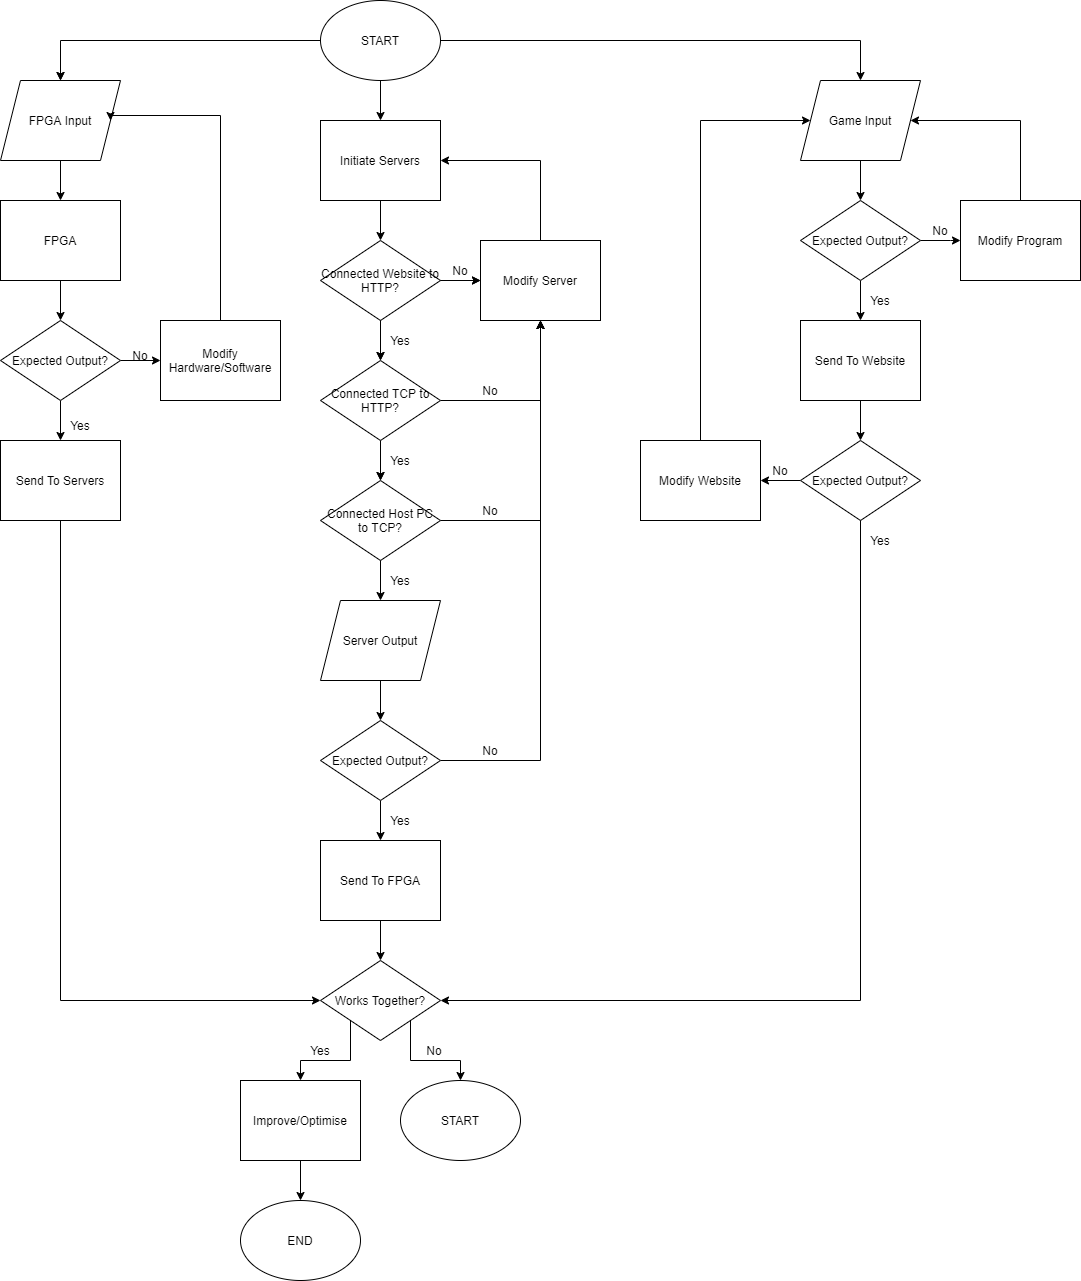
\includegraphics[scale = 0.25]{Flowchart.png}
\end{figure}

\section{\normalsize Resources}

\begin{figure} [h!]
    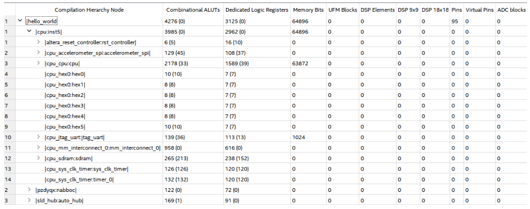
\includegraphics[scale = 0.6]{Res1.png}
    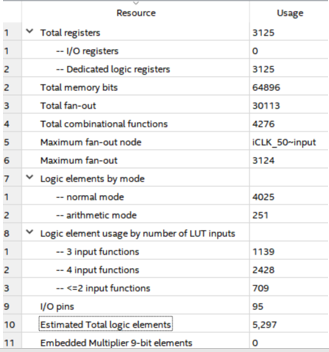
\includegraphics[scale = 0.6]{Res2.PNG}
\end{figure}

\section{\normalsize Appendix}

\underline{\scriptsize Entry 1: How to run the game}
\par
{\scriptsize To play the game, one person must start a server on AWS and run the http\_server.js 
file which starts the HTTP server and then start the TCP server by running the 
TCP\_server.js file, again in the same AWS instance (commands: 
node http\_server.js and node TCP\_server.js)
\par
(Note: to run the JavaScript files, the following JavaScript modules must be 
installed: mongodb, express, cors and path by using the 
npm install module\_name command)
\par
After that the players can open a browser and connect to port 3000 of the AWS server 
(so IP:3000 where IP is the address of the AWS server) and then in the browser they 
must click Connect (without changing the default IP address), then on the next page 
click Start and the game will start displaying.
\par
The players must connect their FPGAs to the host PCs via JTAG UART, blast the Quartus 
project onto the FPGAs, build the C project and download the .elf file to the boards. 
Then they must run the host.py script (command: python3 host.py {AWS\_IP}) in a 
terminal. After running the python script, the cars show up in the browser and the 
players can already start steering their cars.
\par
Once the game is running the players need to try to avoid hitting the orange fields. 
If one hits an orange field, they are out of the game. The game can be restarted at 
any time by clicking on the End Game and then the New Game buttons.}

\end{document}